

%----------------------------------------------------------------------------------------

\newpage

\section*{Synthesis of studied processes}{Synthèse des processus étudiés}


\comment[FL]{cela doit arriver avant gpe/prd $\rightarrow \sim$ p 43}

Nous concluons ce chapitre introductif par une synthèse et une mise en perspective des processus d'interaction identifiés par l'analyse théorique, empirique et la littérature. Celle-ci permettra de situer les revues des entreprises de modélisation auxquelles nous procéderons dans le chapitre~\ref{ch:modelinginteractions}, puis pourra être comparée à celle que nous établirons dans le cas des modèles.


\subsubsection*{A view from scales}{Une entrée par les échelles}

Une première entrée pour synthétiser les processus abordés consiste à les considérer par échelle. On a vu qu'une lecture multi-échelle était pertinente, et que celle-ci permettait globalement de dégager des échelles spatiales et temporelles caractéristiques : microscopique, mesoscopique et macroscopique, avec une assez bonne correspondance des échelles spatiales et temporelles. Cette typologie est bien sûr réduite, puisqu'elle simplifie la classe des processus qui pourraient sortir de ces correspondances, par exemple une mobilité à grande échelle, ou une bifurcation du système urbain qui se manifeste rapidement. De même, les processus eux-même multi-échelle (la gouvernance du Grand Paris en est une bonne illustration, mobilisant des niveaux de gouvernance et des enjeux territoriaux à différentes échelles) sont pris en compte de manière simplifiée. L'axe complémentaire à celui des échelles se base sur les ``effets et causes'' : bien que nous restions toujours dans le cadre d'une causalité complexe comme présenté en introduction, on a mis en évidence des processus pour lequel il est possible d'identifier un précurseur parmi le réseau ou le territoire (nous les noterons alors $A \rightarrow B$), d'autres sont intrinsèquement complexes et contiennent déjà des causalités circulaires (par exemple dans le cas des processus de gouvernance), nous les noterons Réseaux $\leftrightarrow$ Territoires. Le tableau de synthèse est alors donné ci-dessous.


%%%%%%%%%%%%%
\begin{table}[h!]
\begin{tabular}{|l|p{5cm}|p{5cm}|p{5cm}|}
\hline
 & Réseaux $\rightarrow$ Territoires & Territoires $\rightarrow$ Réseaux & Réseaux $\leftrightarrow$ Territoires\\ \hline
Micro & Motifs de mobilité & Congestion du réseau ; Externalités négatives & Mobilité et structure sociale \\ \hline
Meso & Relocalisations ; Effets locaux des infrastructures & Rupture de potentiel & Planification métropolitaine ; TOD \\ \hline
Macro & Interactions entre villes ; Effet tunnel & Différenciation hiérarchique de l'accessibilité & Planification à grande échelle ; Dynamique structurelle ; Bifurcations\\ \hline
\end{tabular}
\end{table}
%%%%%%%%%%%%%



\subsubsection*{A hierarchical view}{Une entrée par les acteurs}

% imbrication hierarchique des concepts ? bof

Une deuxième entrée privilégie le rôle des \emph{acteurs}, c'est à dire des agents qui font le territoire. En effet, les problématique liées à la mobilité concernent les agents microscopiques, celles liées à l'accessibilité des acteurs urbains et économiques, celles liées à la planification des acteurs de gouvernance. Cet aspect peut être résumé par le schéma suivant :


%%%%%%%%%%%%%
\begin{figure}[h!]
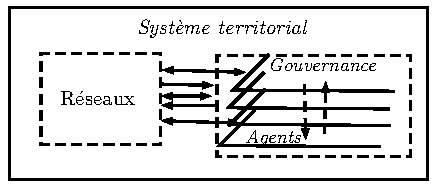
\includegraphics[width=\textwidth]{Figures/Theory/processes_acteurs}
\end{figure}
%%%%%%%%%%%%%


Dans ce schéma, on identifie les acteurs territoriaux au sein du système territorial, qui se déclinent schématiquement sur deux échelles : les agents à l'échelles microscopique qui seront centraux pour les processus de mobilité, et les acteurs de gouvernance à des échelles supérieures, qui mènent les processus de gouvernance. Ils interagissent entre eux de manière complexe, et sont séparés ici conceptuellement par les pointillés d'autre aspects du territoire avec les quels ils sont aussi couplés fortement.


Cette entrée peut être mise en perspective avec le cadre conceptuel de~\cite{le2010approche}, qui étudie les liens entre forme urbaine et pratiques de mobilité dans des contextes métropolitains. Celui-ci comprend le système urbain comme un couplage fort entre système de localisation, système d'activités et système de transport, en précisant l'influence des agents demandeurs (agents micro-économiques) et des agents aménageurs (agents de gouvernance) sur chaque système. Le système de transport correspond à nos réseaux et les deux autres systèmes à un aspect des agents territoriaux, qui contiennent aussi les agents précisés dans ce cadre. Ce parallèle reste à nuancer lorsqu'on change d'échelle : à celle du système de villes, lorsque les agents sont les villes, le système de localisation n'a plus de sens : celui-ci est adapté à une échelle au plus métropolitaine, et surtout aux ontologies correspondantes.


\bigskip

Cette double entrée de lecture des processus d'interaction entre réseaux et territoires conditionnera d'une part la revue de littérature des modèles faite en Chapitre\ref{ch:modelinginteractions}, et sera d'autre part complétée et précisée à l'issue de celui-ci.




%----------------------------------------------------------------------------------------

\newpage


\section*{Chapter Conclusion}{Conclusion du Chapitre}


Les territoires, que nous avons défini comme territoires humains, interagissent de manière complexe avec les réseaux, en particulier ceux de transport, comme montré par les nombreux exemples empiriques ou les constructions théoriques passés en revue. A différentes échelles temporelles typiques, l'année, la décennie et le siècle, correspondent plus ou moins des échelles spatiales : métropolitaine, régionale et système de villes, ainsi que des processus : mobilité, accessibilité et relocalisations, effets systémiques structurels et bifurcations. Les situations concrètes témoignent de réalités locales déclinés avec différentes nuances, et des processus portant ces processus abstraits avec différents rôles et interactions entre eux. Nous avons dans une première section clarifié cette notion d'interaction entre réseaux de transports et territoires en construisant un cadre théorique qui permet de les considérer comme des composantes du système territorial dans son ensemble. Nous avons alors suggéré une approche par la co-évolution pour tenir compte de cette complexité. Afin de mieux cerner ces notions sur des exemples géographiques concrets, nous avons développé en~\ref{sec:casestudies} deux cas d'étude métropolitain d'actualité, et souligné les certitudes en termes d'impact d'accessibilité pour des projets majeurs d'infrastructures qui s'accompagnent systématiquement d'incertitude en terme de trajectoire du système à plus long terme. Enfin, nous proposons en~\ref{sec:qualitative} une excursion par des éléments de terrain dans le Guangdong, Chine. A ce stade, ayant introduit l'objet d'étude thématique, nous proposons de restreindre la portée des entrées prises sur le sujet, et s'intéresser plus particulièrement aux approches impliquant une modélisation, faisant le choix d'un rôle fondamental du \emph{modèle} (sur lequel nous reviendrons plus en détails par la suite) dans la production de connaissance.


% pour limiter les effets d'intermédiaire qui augmenteraient la distance au terrain géographique réel qui est selon~\cite{lefort2012terrain} déjà très présente dans les études le prenant comme matériau empirique principal,




\stars


%-------------------------



